% !TeX program = xelatex
\documentclass[a4paper]{article}

\input{style/ch_xelatex.tex}
\input{style/scala.tex}

%代码段设置
\lstset{numbers=left,
	basicstyle=\tiny,
	numberstyle=\tiny,
	keywordstyle=\color{blue!70},
	commentstyle=\color{red!50!green!50!blue!50},
	frame=single, rulesepcolor=\color{red!20!green!20!blue!20},
	escapeinside=``
}

\graphicspath{ {images/} }
\usepackage{ctex}
\usepackage{graphicx}
\usepackage{color,framed}%文本框
\usepackage{listings}
\usepackage{caption}
\usepackage{amssymb}
\usepackage{enumerate}
\usepackage{xcolor}
\usepackage{bm} 
\usepackage{lastpage}%获得总页数
\usepackage{fancyhdr}
\usepackage{tabularx}  
\usepackage{geometry}
\usepackage{minted}
\usepackage{graphics}
\usepackage{subfigure}
\usepackage{float}
\usepackage{pdfpages}
\usepackage{pgfplots}
\pgfplotsset{width=10cm,compat=1.9}
\usepackage{multirow}
\usepackage{footnote}
\usepackage{booktabs}

%------------------------代码-------------------
\usepackage{xcolor} 
\usepackage{listings} 
\lstset{ 
	language=Verilog, % 设置默认语言为Verilog
	breaklines,%自动换行
	basicstyle=\small\ttfamily, % 使用等宽字体
	escapeinside=``,
	keywordstyle=\color{ blue!70} \bfseries,
	commentstyle=\color{red!50!green!50!blue!50},% 
	stringstyle=\ttfamily,% 
	extendedchars=false,% 
	linewidth=\textwidth,% 
	numbers=left,% 
	numberstyle=\tiny \color{blue!50},% 
	frame=trbl,% 
	rulesepcolor= \color{ red!20!green!20!blue!20} 
}

%-------------------------页面边距--------------
\geometry{a4paper,left=2.3cm,right=2.3cm,top=2.7cm,bottom=2.7cm}
%-------------------------页眉页脚--------------
\usepackage{fancyhdr}
\pagestyle{fancy}
\lhead{\kaishu \leftmark}
% \chead{}
\rhead{\kaishu 计算机网络实验报告}%加粗\bfseries 
\lfoot{}
\cfoot{\thepage}
\rfoot{}
\renewcommand{\headrulewidth}{0.1pt}  
\renewcommand{\footrulewidth}{0pt}%去掉横线
\newcommand{\HRule}{\rule{\linewidth}{0.5mm}}%标题横线
\newcommand{\HRulegrossa}{\rule{\linewidth}{1.2mm}}
\setlength{\textfloatsep}{10mm}%设置图片的前后间距
%--------------------文档内容--------------------

\begin{document}
	\renewcommand{\contentsname}{目\ 录}
	\renewcommand{\appendixname}{附录}
	\renewcommand{\appendixpagename}{附录}
	\renewcommand{\refname}{参考文献} 
	\renewcommand{\figurename}{图}
	\renewcommand{\tablename}{表}
	\renewcommand{\today}{\number\year 年 \number\month 月 \number\day 日}
	
	%-------------------------封面----------------
	\begin{titlepage}
		\begin{center}
			
\includegraphics[width=0.8\textwidth]{NKU.png}\\[1cm]
			\vspace{20mm}
				\textbf{\huge\textbf{\kaishu{计算机学院}}}\\[0.5cm]
				\textbf{\huge{\kaishu{计算机网络实验报告}}}\\[2.3cm]
				\textbf{\Huge\textbf{\kaishu{配置Web服务器，捕获HTTP报文并分析}}}
			
			\vspace{\fill}
			
			% \textbf{\Large \textbf{计算机网络实验报告}}\\[0.8cm]
			% \HRule \\[0.9cm]
			% \HRule \\[2.0cm]
			\centering
				\textsc{\LARGE \kaishu{姓名\ :\ 王一诺}}\\[0.5cm]
				\textsc{\LARGE \kaishu{学号\ :\ 2312331}}\\[0.5cm]
				\textsc{\LARGE \kaishu{专业\ :\ 计算机科学与技术}}\\[0.5cm]
			
			\vfill
			{\Large \today}
		\end{center}
	\end{titlepage}
	
	\renewcommand {\thefigure}{\thesection{}.\arabic{figure}}%图片按章标号
	\renewcommand{\figurename}{图}
	\renewcommand{\contentsname}{目录}  
	\cfoot{\thepage\ of \pageref{LastPage}}%当前页 of 总页数
	
	
	% 生成目录
	\clearpage
	\tableofcontents
	\newpage
	\setcounter{figure}{0} % 每章开始前重置图片计数器
	
	
	\section{实验要求与任务}
	配置Web服务器，捕获HTTP报文并分析，实验要求：
	\begin{enumerate}
		\item 搭建Web服务器（自由选择系统），并制作简单的Web页面，包含简单文本信息（包含专业、学号、姓名）和6幅图像。
		\item 通过浏览器获取自己编写的Web页面，使用Wireshark捕获浏览器与Web服务器的交互过程。
		\item 分析两个报文的封装层次，包括数据链路层、互连层、传输层、应用层。
		\item 对整个HTTP交互过程进行详细说明，使用Wireshark过滤器使其仅显示HTTP协议。
		\item 提交HTML文档、Wireshark捕获文件和实验报告。
	\end{enumerate}
	
	\section{Web 服务器搭建}
	本次实验通过 python -m http.server 8000 启动了纯 HTTP 的简易 Web 服务器，监听在 localhost:8000 ，未启用 HTTPS 或任何反向代理，从浏览器访问 http://localhost:8000/index.html 即可直接获取页面内容。服务器无额外路由和压缩配置，所有资源均为本地静态文件，这种极简架构方便 Wireshark 抓取到完整的明文请求行、响应行以及头部和实体，对后续报文分析提供了清晰数据。
	
	编写了 index.html，HTML 结构扁平清晰：<header> 仅呈现标题“Networking Lab 3 Page”，<main> 内的 .card 区块承载实验要求的基本文本信息，使用 <ul> 列表列出专业、学号、姓名等字段。页面使用内联样式保证背景、卡片、文字和分隔线的基础视觉效果，但未引入复杂脚本或外链资源，确保页面保持不要太复杂，减少额外 HTTP 请求。

	页面下半部分的 <div class="gallery"> 构成六宫格图像区域，逐一引用 images/pic1.svg 至 images/pic6.svg 六个本地 SVG 文件，每个 <figure> 内包含 <img> 与 <figcaption>，带有描述性 alt 文本和文字说明，保证可访问性与语义清晰度。六幅图像均为静态本地资源，无外部依赖，浏览器在加载 index.html 后会顺序发起六个独立的 HTTP GET 请求，便于在抓包时观察多对象的并行获取过程和缓存行为。

	设计完成后，在当前文件夹下运行指令 python -m http.server 8000 并打开浏览器访问 http://localhost:8000/index.html ，可以看到：

	\begin{figure}[H]
		\centering
		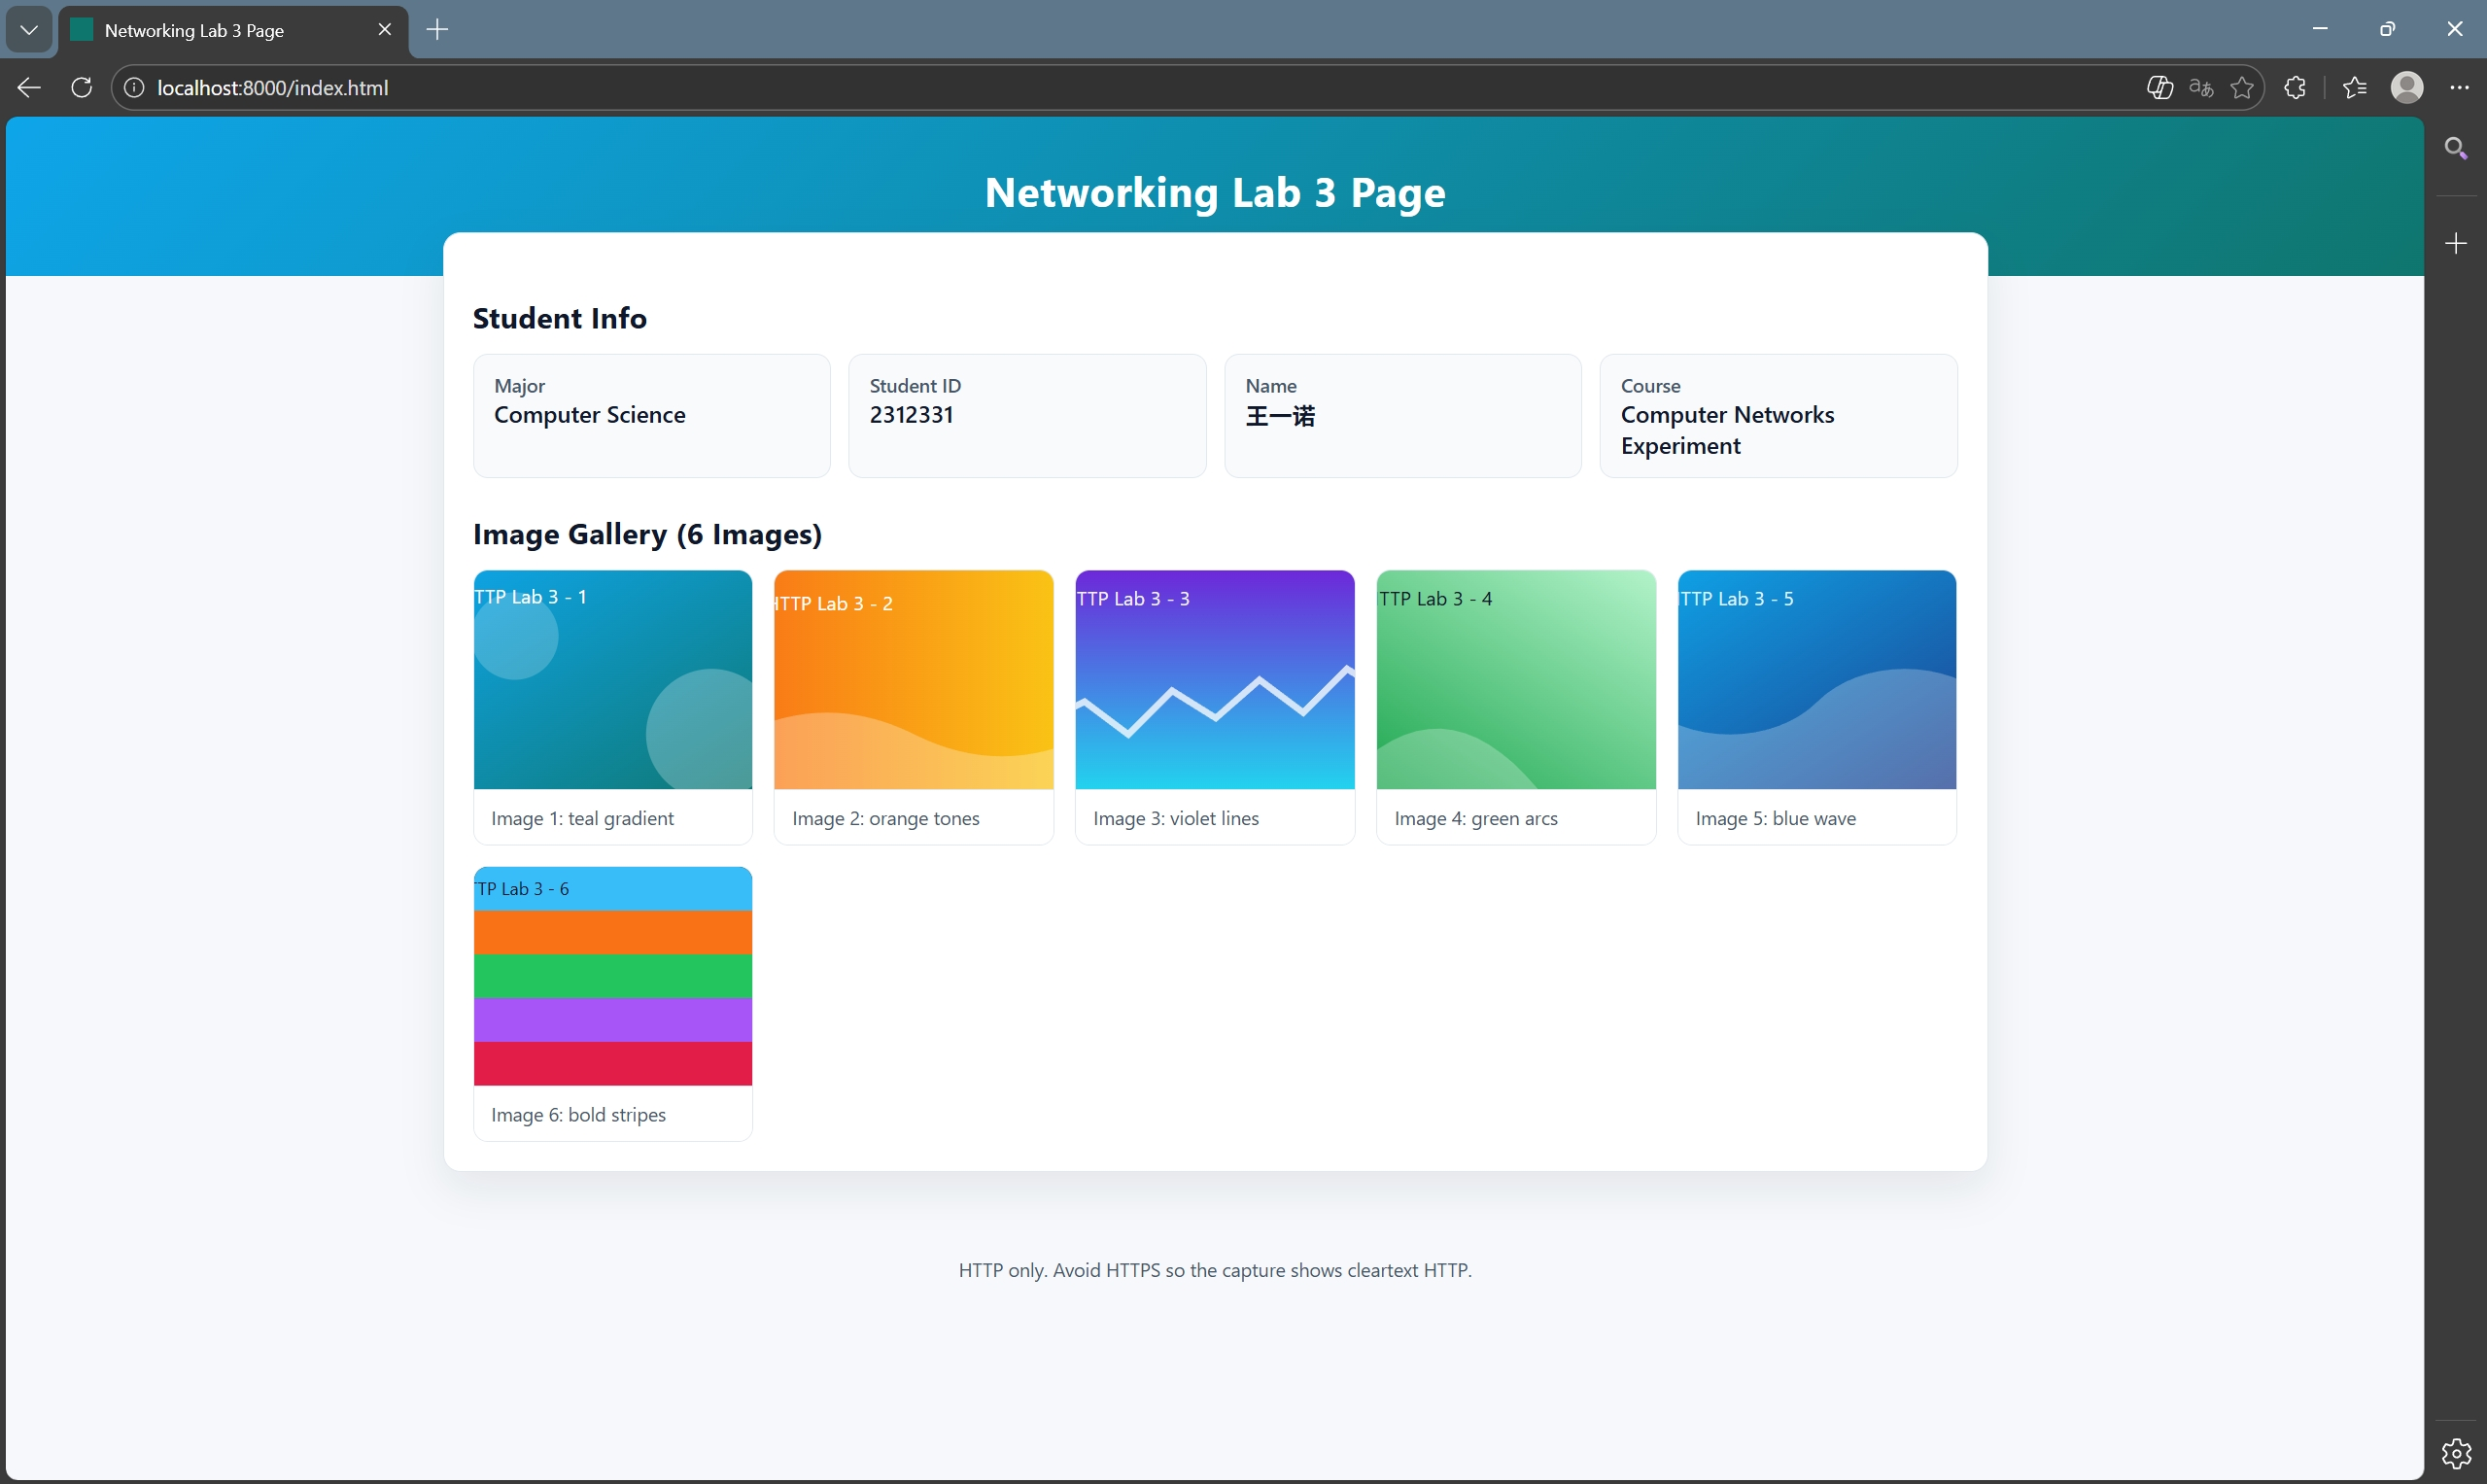
\includegraphics[width=\textwidth]{web.png}
		\caption{web页面截图}
	\end{figure}

	\section{Wireshark抓包}
	终端进入网页目录启动 HTTP 服务 python -m http.server 8000 后，使用 Wireshark 抓取本地回环接口的数据包，设置过滤器 tcp port 8000 后打开浏览器访问 http://localhost:8000/index.html ，浏览器会发送 HTTP GET 请求获取网页及其六幅图像资源，Wireshark 会捕获到这些明文 HTTP 报文，如下图所示：

	\begin{figure}[H]
		\centering
		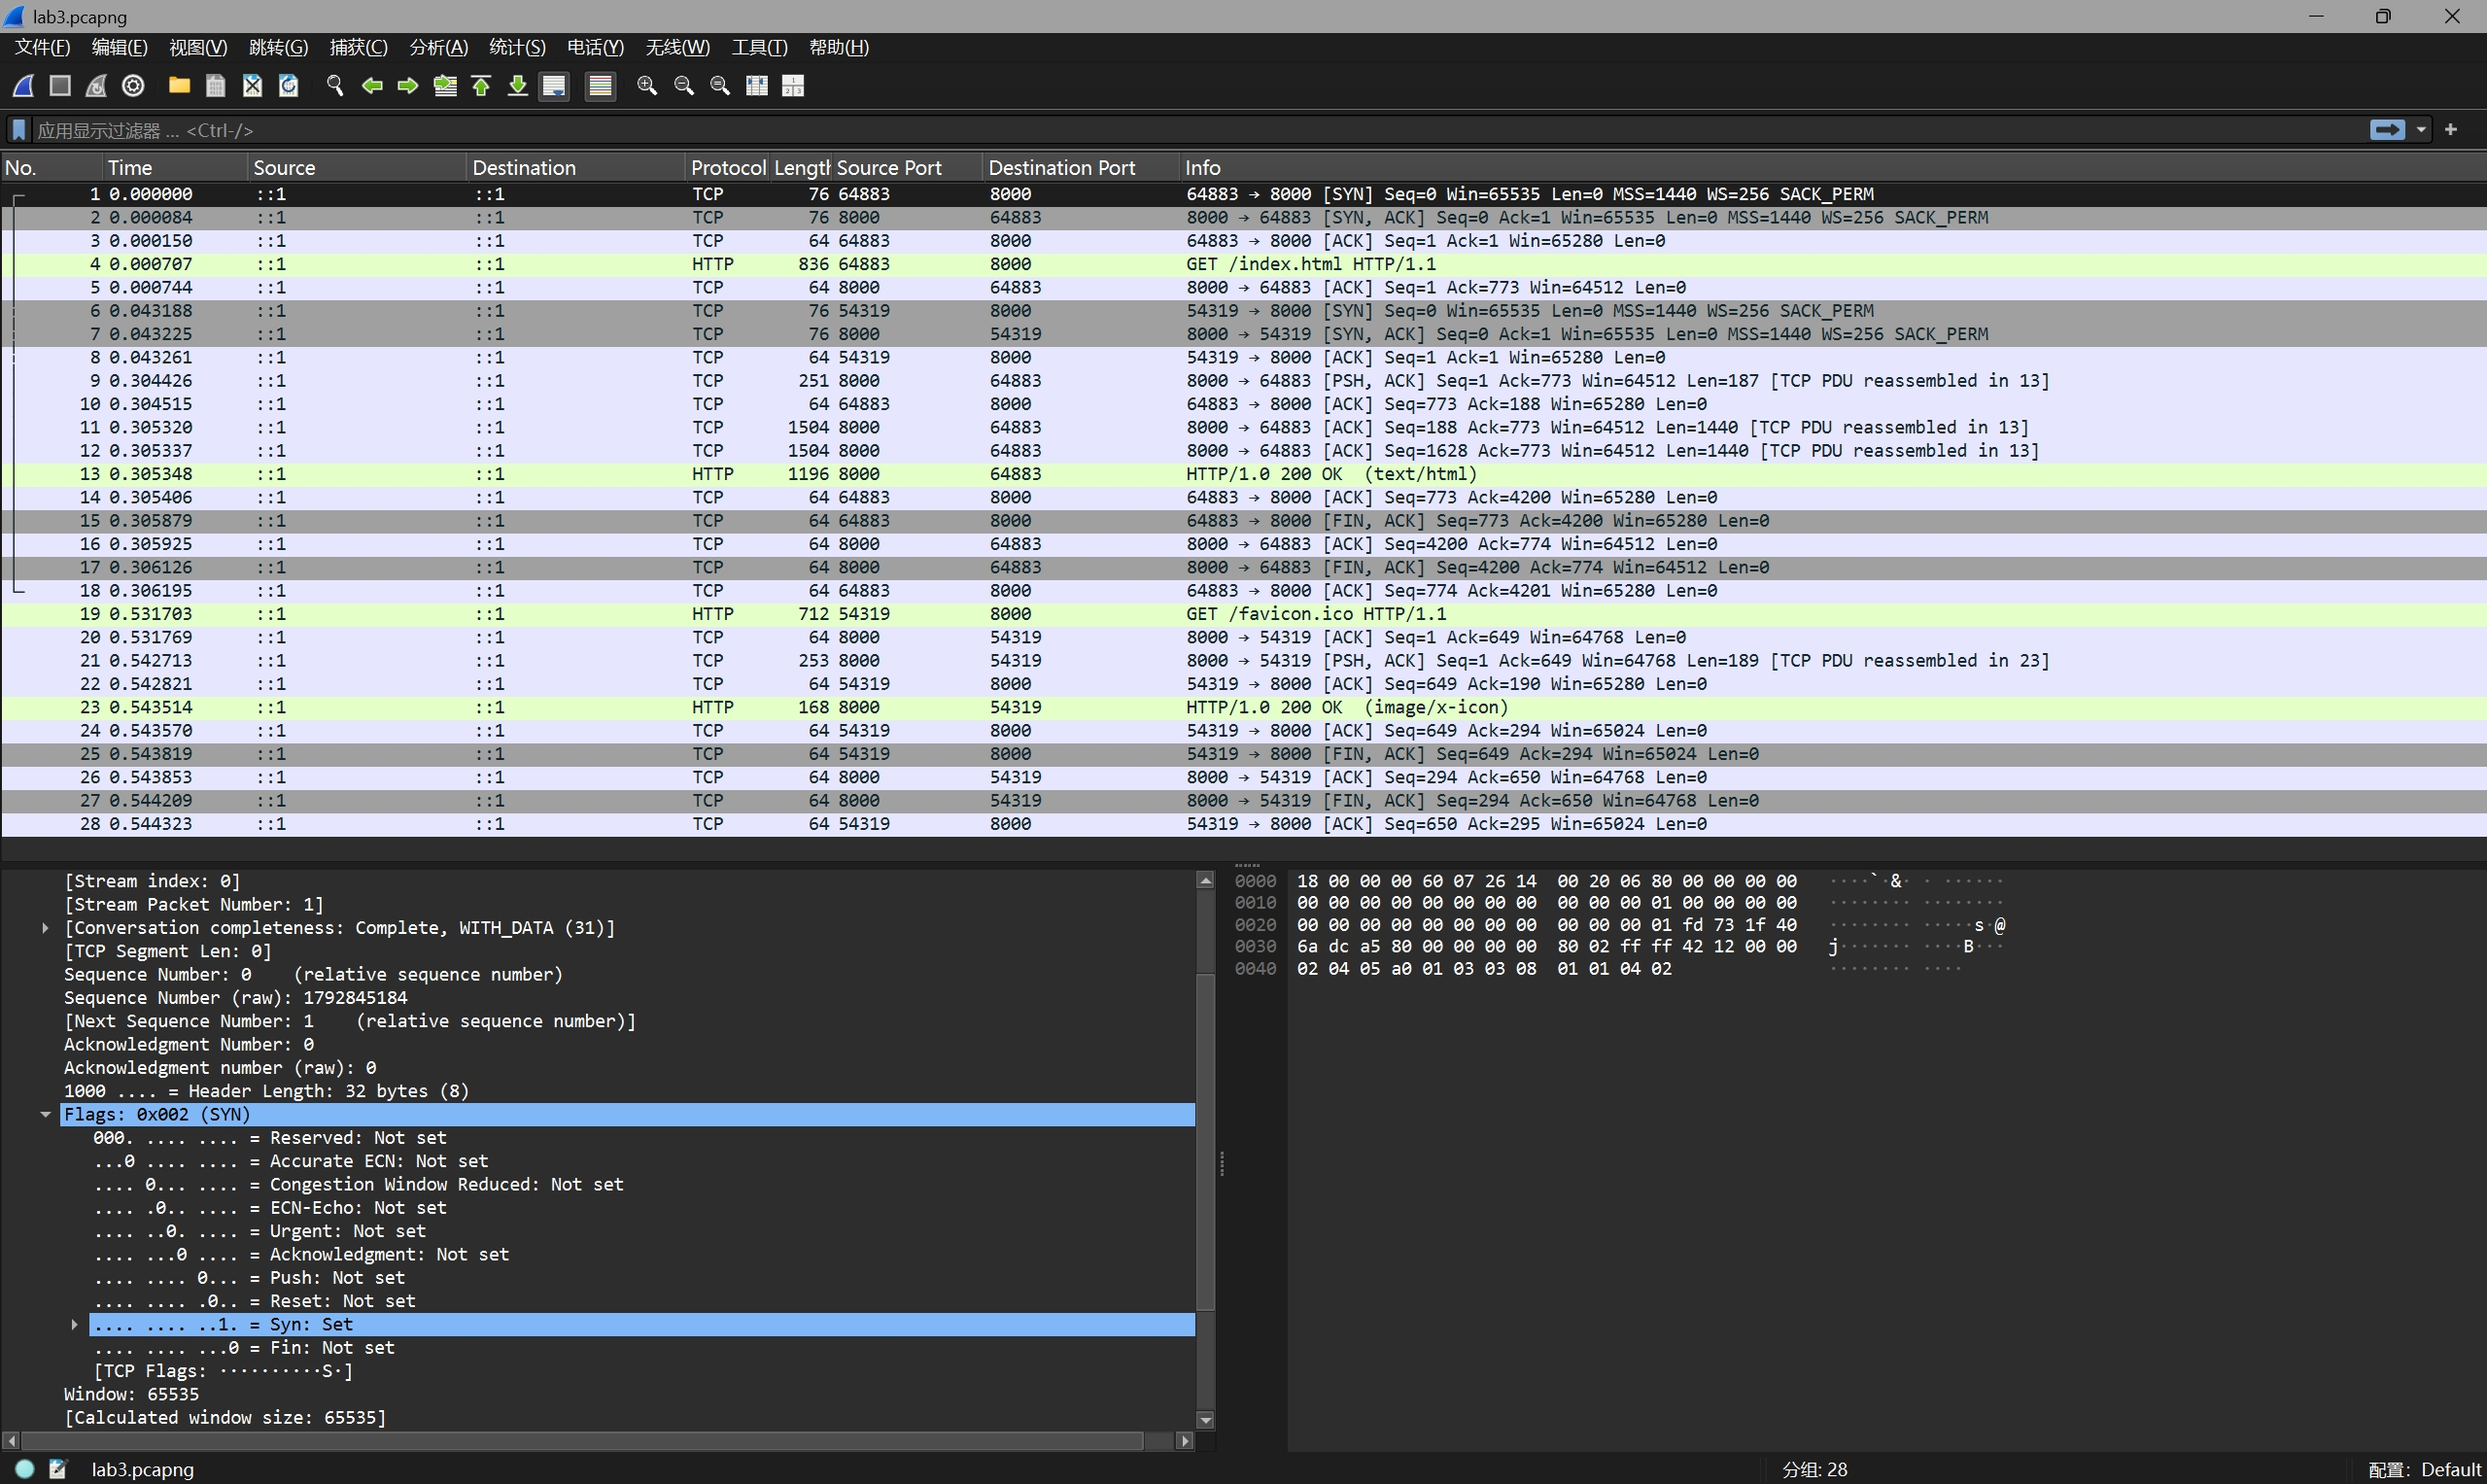
\includegraphics[width=\textwidth]{ws.png}
		\caption{Wireshark抓包}
	\end{figure}

	我们可以先简单的逐条观察一下这些报文，它们大致可以分成两部分：

	\subsection{连接 A：获取 index.html 页面}
	第一部分是客户端端口 64883 → 服务端 8000，请求 index.html的报文：
	\begin{itemize}
		\item \texttt{报文 idx0 SYN}: 链路层是 Loopback 伪头，无源/目的 MAC；网络层为 IPv6，源 `::1`、目的 `::1`，载荷指向 TCP；传输层 TCP 源端口 64883 → 8000，SYN=1、Seq=1792845184、窗口 65535，无负载；应用层无内容，开启三次握手。
		\item \texttt{报文 idx1 SYN/ACK}: 仍是 Loopback+IPv6；服务器 8000 → 客户端 64883，SYN/ACK 置位，Seq=1737695183，Ack=1792845185（对客户端 SYN+1 确认），窗口 65535；无应用数据，回应握手。
		\item \texttt{报文 idx2 ACK}: 客户端 64883 → 8000，ACK 置位，Seq=1792845185，Ack=1737695184，窗口 255；完成三次握手，连接建立，应用层仍为空。
		\item \texttt{报文 idx3 HTTP GET}: 客户端首个带数据报文，IPv6 载 TCP PSH/ACK，Seq=1792845185，Ack=1737695184，负载 772 字节；应用层为明文 `GET /index.html HTTP/1.1`，Host 为 `localhost:8000`，包含 UA、Accept、Accept-Language、If-Modified-Since 等请求头，表明浏览器要拉取主页。
		\item \texttt{报文 idx4 ACK}: 服务器对上述 GET 的纯确认，Seq=1737695184，Ack=1792845957（对 772 字节请求的累积确认），窗口 252，无应用数据。
		\item \texttt{报文 idx8 HTTP/1.0 200 OK 首部}: 服务器发回首个响应报文，PSH/ACK，Seq=1737695184，Ack=1792845957，负载 187 字节；应用层是 `HTTP/1.0 200 OK` 响应头，Server=SimpleHTTP/0.6 Python/3.12.7，Content-Type=text/html，Content-Length=4012。
		\item \texttt{报文 idx9 ACK}: 客户端对响应头的确认，Seq=1792845957，Ack=1737695371，无数据；通知服务器已收到 187 字节。
		\item \texttt{报文 idx10 HTML 数据段 1}: 服务器继续下发主体，ACK 置位（无 PSH），Seq=1737695371，Ack=1792845957，负载 1440 字节；内容为 HTML 开头、CSS 等，属于 `index.html` 的正文第一段。
		\item \texttt{报文 idx11 HTML 数据段 2}: 同一连接继续传输，Seq=1737696811，Ack=1792845957，负载 1440 字节；仍是页面主体的中间部分（样式、排版）。
		\item \texttt{报文 idx12 HTML 数据段 3（收尾）}: 服务器最后一段数据，PSH/ACK，Seq=1737698251，Ack=1792845957，负载 1132 字节；包含页面中个人信息与 6 张图片 `<img>` 标签区域以及页脚提示，标志正文发送完毕。
		\item \texttt{报文 idx13 ACK}: 客户端确认全部 HTML 数据，Seq=1792845957，Ack=1737699383，无数据；服务器窗口继续开放。
		\item \texttt{报文 idx14 FIN/ACK（客户端）}: 浏览器主动关闭该 TCP 连接，Seq=1792845957，Ack=1737699383，FIN=1、ACK=1，无负载；表示主页内容收取完成。
		\item \texttt{报文 idx15 ACK（服务器对 FIN）}: 服务器确认客户端的 FIN，Seq=1737699383，Ack=1792845958，无数据；准备半关闭。
		\item \texttt{报文 idx16 FIN/ACK（服务器）}: 服务器发送自己的 FIN，Seq=1737699383，Ack=1792845958，FIN=1、ACK=1，无负载；请求关闭方向。
		\item \texttt{报文 idx17 最终 ACK}: 客户端对服务器 FIN 的确认，Seq=1792845958，Ack=1737699384，无数据；连接 A 四次挥手结束。
	\end{itemize}

	\subsection{连接 B：获取 favicon.ico 图标}
	第二部分是客户端端口 54319 → 服务端 8000，请求 favicon.ico 的报文：

	\begin{itemize}
		\item \texttt{报文 idx5 SYN}：Loopback+IPv6，同样是新建 TCP 连接，客户端端口 54319，Seq=4172531794，窗口 65535，SYN=1，无应用负载。
		\item \texttt{报文 idx6 SYN/ACK}：服务器 8000 → 54319，SYN/ACK，Seq=2706956766，Ack=4172531795，窗口 65535；握手第二步。
		\item \texttt{报文 idx7 ACK}：客户端 ACK，Seq=4172531795，Ack=2706956767，窗口 255；握手完成，连接 B 建立。
		\item \texttt{报文 idx18 HTTP GET /favicon.ico}：客户端发送 PSH/ACK，Seq=4172531795，Ack=2706956767，负载 648 字节；应用层请求行 `GET /favicon.ico HTTP/1.1`，Host=localhost:8000，Accept 为多种图片类型，Referer 指向 `/index.html`，说明浏览器自动取图标。
		\item \texttt{报文 idx19 ACK}：服务器确认 GET 请求，Seq=2706956767，Ack=4172532443，无数据；表明收到了 648 字节。
		\item \texttt{报文 idx20 HTTP 200 图标首部}：服务器 PSH/ACK，Seq=2706956767，Ack=4172532443，负载 189 字节；应用层为 `HTTP/1.0 200 OK` 响应头，Content-Type=image/x-icon，Content-Length=104。
		\item \texttt{报文 idx21 ACK}：客户端确认响应头，Seq=4172532443，Ack=2706956956，无数据；准备接收图标主体。
		\item \texttt{报文 idx22 图标数据}：服务器发送 PSH/ACK，Seq=2706956956，Ack=4172532443，负载 104 字节；负载开头为 PNG/Ico 二进制模数，即 `favicon.ico` 的文件内容。
		\item \texttt{报文 idx23 ACK}：客户端确认图标数据，Seq=4172532443，Ack=2706957060，无数据；所有有效载荷已收完。
		\item \texttt{报文 idx24 FIN/ACK（客户端）}：浏览器主动关闭图标连接，Seq=4172532443，Ack=2706957060，FIN=1、ACK=1，无负载。
		\item \texttt{报文 idx25 ACK（服务器对 FIN）}：服务器确认客户端 FIN，Seq=2706957060，Ack=4172532444，无数据。
		\item \texttt{报文 idx26 FIN/ACK（服务器）}：服务器发送自己的 FIN，Seq=2706957060，Ack=4172532444，FIN=1、ACK=1，无负载。
		\item \texttt{报文 idx27 最终 ACK}：客户端对服务器 FIN 的确认，Seq=4172532444，Ack=2706957061，无数据，连接 B 释放。
	\end{itemize}

	\subsection{简单概括}
	大眼过一遍这些报文，可以简单概括一下交互过程：
	\begin{itemize}
		\item 浏览器首先发起连接 A 完成三次握手（idx0–2），发送 `GET /index.html` 请求（idx3），服务器分四段回送 HTTP/1.0 200 OK 及 4012 字节 HTML 正文（idx8、10、11、12），客户端确认后主动挥手关闭（idx14–17）。这一过程展示了 TCP 建立、可靠传输（多段 ACK 确认）、以及四次挥手的完整流程。
		\item 浏览器随后为站点图标开启独立的连接 B（idx5–7），发送 `GET /favicon.ico`（idx18），服务器回 200 OK 响应头与 104 字节图标数据（idx20、22），客户端同样在数据收齐后主动关闭（idx24–27）。这体现了浏览器并行复用多个 TCP 连接获取资源的行为。
		\item 全部报文在 Wireshark 使用显示过滤器 `http` 即可呈现仅 HTTP 相关的 TCP 报文；链路层为本机 Loopback，网络层为 IPv6 本地回环 `::1`，传输层为 TCP 可靠传输，应用层为明文 HTTP，无 TLS 加密，便于观察请求行、响应头与正文内容。
	\end{itemize}

	\section{报文的封装层次}
	接下来，我们选择两个典型报文进行封装层次分析：报文 A 为客户端请求主页的 HTTP GET 报文（idx3），报文 B 为服务器响应主页的 HTTP/1.0 200 OK 报文（idx8）。下面分别对这两个报文在数据链路层、互连层、传输层和应用层的封装内容进行详细说明。

	\subsection{报文 A（GET /index.html）封装层次}
	\begin{figure}[H]
		\centering
		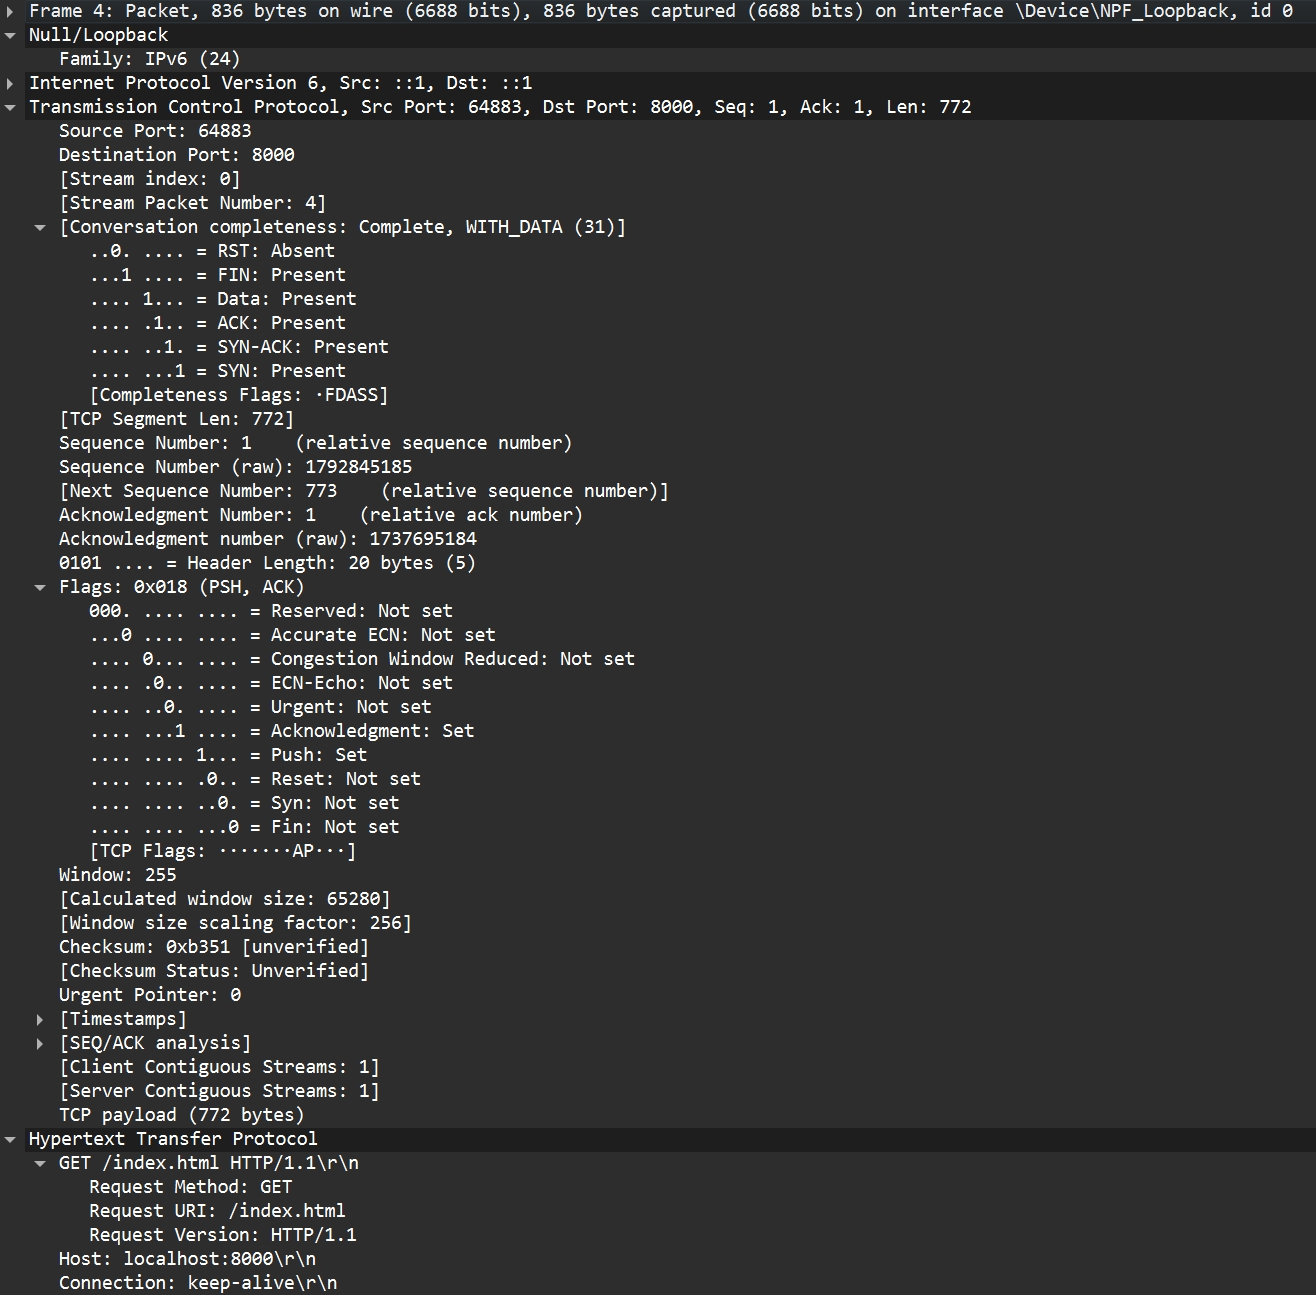
\includegraphics[width=\textwidth]{A.png}
		\caption{报文 A}
	\end{figure}

	\paragraph{数据链路层}：抓包链路类型为 pcapng linktype 0（Loopback），无以太网头，开头 4 字节协议标识表明上层是 IPv6；因此无源/目的 MAC，链路只负责本机回环的“虚拟交付”。

	\paragraph{互连层（IPv6）}：版本号 6，源地址 `::1`、目的地址 `::1`，流标签与分类字段保持默认，跳数限制 TTL（Hop Limit）为常规本地值，净荷长度指向 TCP 负载；此层提供无连接的分组传递与寻址，本实验中为回环寻址，等价“自发自收”。

	\paragraph{传输层（TCP）}：源端口 64883，目的端口 8000，Seq=1792845185，Ack=1737695184，窗口 255，标志位 PSH+ACK——表明携带上层数据且对前一报文确认，头部长度 20 字节，无选项；TCP 在此层提供可靠、按序、无差错的字节流并维护序列号/确认号、窗口与重传控制。

	\paragraph{应用层（HTTP 请求）}：明文 `GET /index.html HTTP/1.1`，Host: localhost:8000；包含 UA、Accept、Accept-Language、If-Modified-Since 等头；这一层定义浏览器与服务器的语义交互（请求方法、资源路径、首部协商），依赖下层 TCP 的可靠传输保证请求完整送达。

	\subsection{报文 B（HTTP/1.1 200 OK）封装层次}
	\begin{figure}[H]
		\centering
		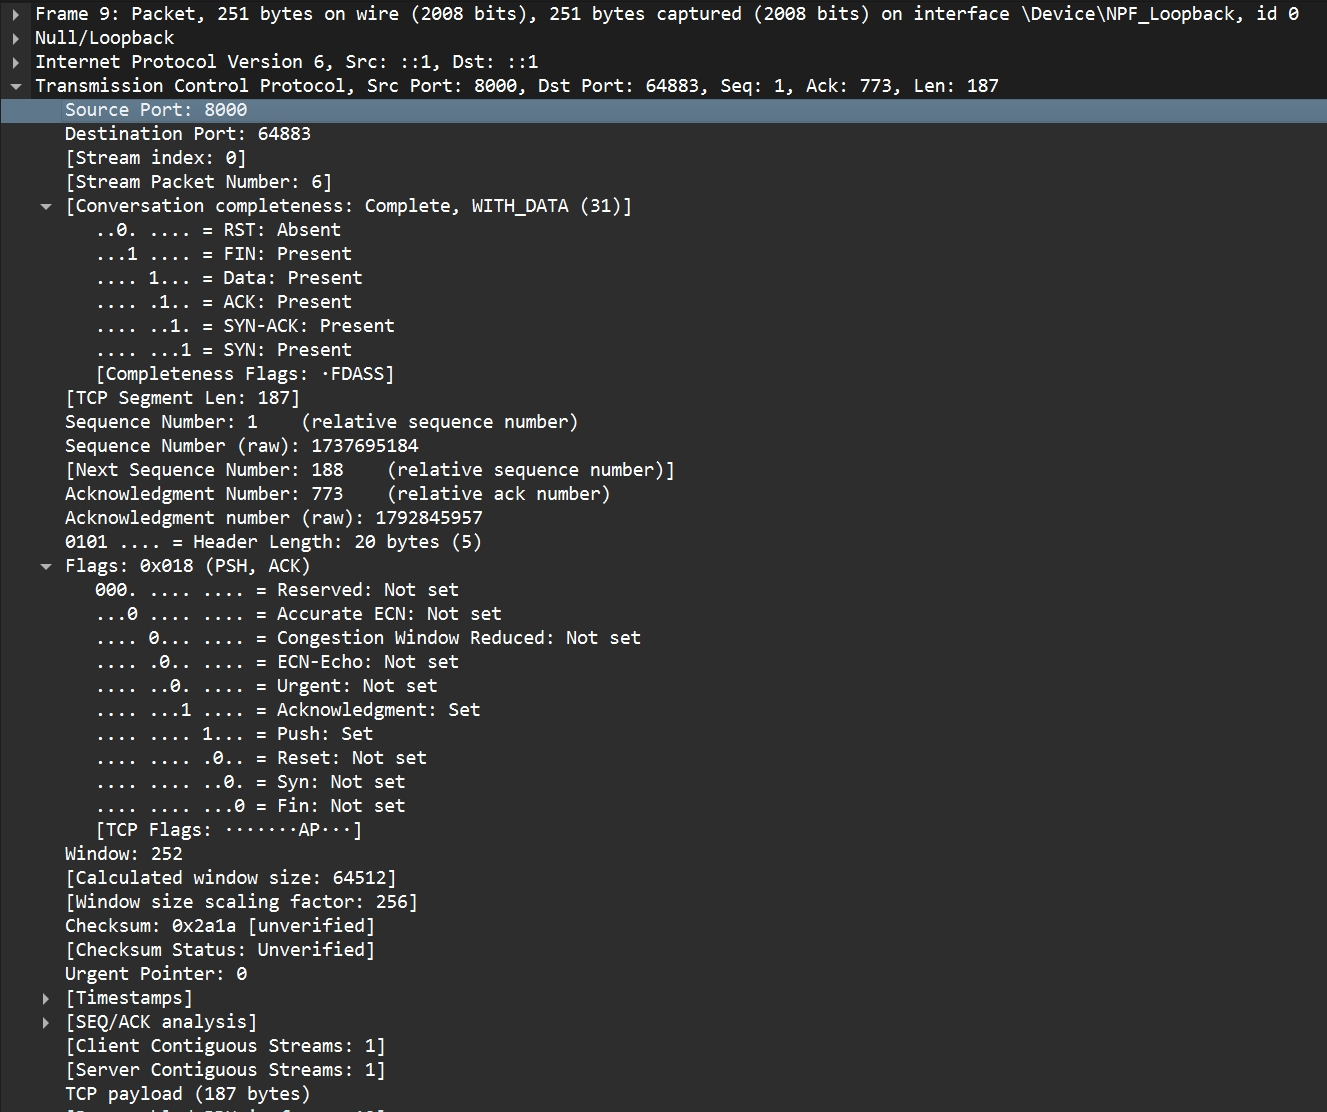
\includegraphics[width=\textwidth]{B.png}
		\caption{报文 B}
	\end{figure}

	\paragraph{数据链路层}：同样是 Loopback 伪链路头，linktype 0，4 字节协议标识指向 IPv6，无真实 MAC，说明报文仅在本机栈内回环传递。

	\paragraph{互连层（IPv6）}：源地址 `::1`、目的地址 `::1`，版本 6，净荷长度覆盖 TCP 段，Hop Limit 为本地默认；该层为上层 TCP 提供分组封装与路由。

	\paragraph{传输层（TCP）}：源端口 8000，目的端口 64883，Seq=1737695184，Ack=1792845957，窗口 252，标志位 PSH+ACK，负载 187 字节；此报文既确认客户端请求字节，也携带上层 HTTP 响应首部，体现 TCP 的可靠交付与流量控制（窗口值）。

	\paragraph{应用层（HTTP 响应）}：`HTTP/1.0 200 OK`，Server: SimpleHTTP/0.6 Python/3.12.7，Date: Wed, 31 Dec 2025 10:24:52 GMT，Content-Type: text/html，Content-Length: 4012，Last-Modified: Wed, 31 Dec 2025 09:42:48 GMT；应用层说明服务器成功处理 GET 请求并返回正文长度/类型等元数据，为浏览器后续接收完整 HTML 正文做准备。

	\subsection{小结}
	两条报文展示了典型的四层封装：Loopback 伪链路头（替代以太网）、IPv6 分组（提供寻址与分片前准备）、TCP 段（可靠传输与确认/窗口机制）、HTTP 文本（语义请求/响应）。在 Wireshark 中逐层展开可清晰看到每层头字段如何配合：链路层确定上层协议，IP 层确定源/目的与分组长度，TCP 层用序号/确认号/窗口保障可靠流，HTTP 层承载具体业务语义。
	
	\section{HTTP交互过程总结}
	本次实验通过搭建简易 HTTP 服务器并使用 Wireshark 抓包，完整捕获了浏览器与服务器之间的 HTTP 交互过程。以下是对该过程的详细总结：
	\subsection{交互过程}
	按时间顺序依次是：
	\begin{itemize}
		\item 浏览器先对主页连接发起三次握手（idx0–2），SYN、SYN/ACK、ACK 依次完成，未携带应用数据。
		\item 客户端发送 HTTP GET /index.html（idx3），TCP 标志 PSH+ACK，Seq=1792845185，Ack=1737695184，负载 772 字节请求头。
		\item 服务器回纯 ACK（idx4），确认收到全部请求字节，准备发送响应。
		\item 服务器发送 200 OK 首部（idx8），PSH+ACK，Seq=1737695184，Ack=1792845957。
		首部声明 Content-Type=text/html、Content-Length=4012。
		Last-Modified 及 Server=SimpleHTTP/0.6 Python/3.12.7 一并给出。
		\item 客户端 ACK 首部（idx9），确认后续等待正文。
		\item 服务器分段发送 HTML 正文（idx10、idx11、idx12），分别 1440、1440、1132 字节。
		idx10、idx11 为 ACK 置位，包含 HTML 头部与 CSS。
		idx12 为 PSH+ACK，收尾段含个人信息区、6 张图片标签和页脚提示。
		\item 客户端累积 ACK（idx13），Ack=1737699383，确认正文收齐。
		服务器窗口保持开放，为后续关闭做准备。
		\item 客户端发起关闭（idx14），FIN/ACK 表示主页内容收完。
		服务器回 ACK 再发 FIN/ACK（idx15、idx16），客户端最终 ACK（idx17）。
		四次挥手完成，主页连接释放。
		\item 浏览器为图标建立第二条连接（idx5–7），重复 SYN、SYN/ACK、ACK。
		\item 客户端发送 GET /favicon.ico（idx18），PSH+ACK，负载 648 字节。
		请求头包含 Host=localhost:8000，Referer=/index.html，说明为同站资源。
		\item 服务器回纯 ACK（idx19），确认收到图标请求。
		\item 服务器返回图标响应头（idx20），PSH+ACK，Content-Type=image/x-icon，Content-Length=104。
		发送 104 字节图标主体（idx22），客户端在 idx21 与 idx23 ACK。
		\item 客户端主动关闭图标连接（idx24），服务器先 ACK。
		服务器再发 FIN/ACK（idx25、idx26），客户端最终 ACK（idx27），四次挥手完成。
	\end{itemize}

	\subsection{过程特征与说明}
	\begin{itemize}
		\item \textbf{多连接并行}：主页与图标各占一条 TCP 连接，符合浏览器并行取资源行为。
		\item \textbf{TCP 可靠性}：每段数据都有 ACK，序列号与负载长度匹配，四次挥手完整呈现连接释放。
		\item \textbf{HTTP 明文}：使用 http，未加密，内容直接可见。
		\item \textbf{链路与网络层简化}：Loopback 伪头，无以太网；IPv6 回环 `::1`，无路由跳转。
		\item \textbf{应用层元数据}：Content-Length、Content-Type 指定正文长度与类型；User-Agent、Accept、Referer 说明客户端能力和来源。
	\end{itemize}
	
	\section{实验总结与改进方向}
	通过本次实验，我深入理解了 HTTP 协议的工作原理及其在 TCP/IP 四层模型中的封装过程。搭建简易 Web 服务器并使用 Wireshark 抓包，能够直观地观察到浏览器与服务器之间的交互细节，包括请求行、响应头以及数据传输的可靠性机制。

	实验过程中，更具体深入地掌握了以下知识点：
	\begin{itemize}
		\item HTTP 请求与响应的结构和语义，理解了常用方法（如 GET）及状态码（如 200 OK）的含义。
		\item TCP 三次握手和四次挥手的过程，了解了连接建立与释放的机制。
		\item Wireshark 的使用技巧，包括过滤器设置和报文分析方法，能够有效地捕获和解读网络数据包。
		\item HTTP 报文在数据链路层、互连层、传输层和应用层的封装细节，理解了各层协议的作用和协同工作方式。
		\item 浏览器多连接并行获取资源的行为，认识到现代浏览器在性能优化方面的设计。
		\item 本地回环接口的网络通信特点，理解了 Loopback 伪链路和 IPv6 回环地址的应用场景。
		\item HTTP 明文传输的安全隐患，认识到在实际应用中应使用 HTTPS 进行加密保护。
		\item 服务器响应头中的元数据作用，如 Content-Length 和 Content-Type 对客户端处理数据的重要性。
	\end{itemize}
	
\end{document}
